\Chapter{Az OpenCL szabvány bemutatása}

\Section{Az OpenCL szabvány eredete}

A jelenlegi világban több platform is képes párhuzamosságra, ilyenek például a CPU, GPU, DSP \cite{dsp}, vagy FPGA \cite{fpga} processzor és egyebek, és ezekre mind létezik specifikus párhuzamos programozási módszer, mint az OpenMP \cite{openmp}, MPI \cite{mpi}, hibrid módszerek \cite{hybrid}, specifikus könyvtárak, de ezek csak az adott platformon működnek, egy MPI program nem futtatható egy videókártyán. Ezért volt szükség egy heterogén platformra, ami áthidalja a különböző platformokat és egy egységes programozói felületet biztosít (\ref{fig:openCl} ábra).

\begin{figure}[h]
\centering
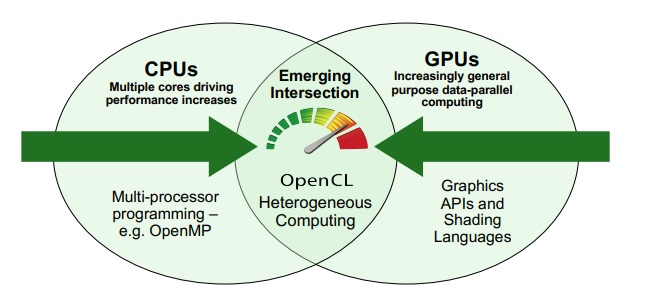
\includegraphics[scale=0.7]{images/opencl_origin.jpg}
\caption{Az OpenCL létrejötte. \cite{opencl_origin}}
\label{fig:openCl}
\end{figure}

A legnagyobb gyártók így összefogtak, nemcsak az OpenCL, de más, közös célok érdekében létrehozták a Khronos csoportot. A Khronos csoportnak jelenleg több mint 150 tagja van, többek között az AMD, Apple, arm, NVIDIA, Samsung, Google, Intel \cite{khronos_about} \cite{khronos_members}. A csoport alapítása óta sok más nyílt szabványt is létrehozott, mint például a Vulkan \cite{vulkan}, vagy az OpenGL \cite{opengl}. 2008 december 9.én kiadták az OpenCL 1.0 -át és azóta is folyamatosan fejlesztik \cite{opencl1}, 2020 szeptember 30.adikán az OpenCL 3.0 megérkezett \cite{opencl}.

Az új szabvány mögött egy nagy ötlet állt, hogy lecserélik a hagyományos ciklusokat úgynevezett kernelekre, amikből példányokat hozunk létre, munka elemeket, és ezek a munkaelemek egymással párhuzamosan futnak (\ref{fig:loopVsKernel} ábra).

\begin{figure}[h]
\centering
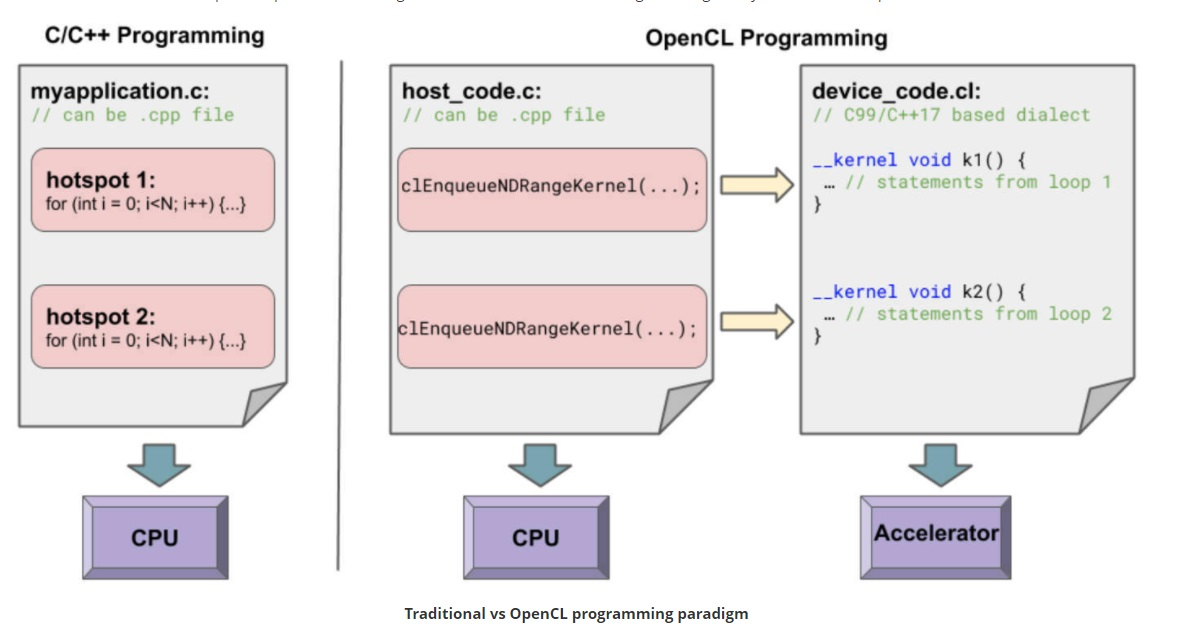
\includegraphics[scale=0.4]{images/loopvskernel.jpg}
\caption{Ciklus <-> Kernel \cite{opencl}}
\label{fig:loopVsKernel}
\end{figure}

A kerneleknek szükségük van egy N dimenziós tartományra ahol a munkájukat végzik, az OpenCL  ezt is specifikálja, ez az NDRange. Egy kernel futtatásakor maximum 3 dimenziót specifikálunk, valamint az adott dimenzió problémáinak, eseteinek számát, méretét, ezt globális méretnek nevezzük. Az adott tartományban minden pontot megfeleltetünk egy munka elemmel, amiket munkacsoportokra osztunk. A munkaelemek egy munkacsoporton belül tudnak egymással kommunikálni, és osztozkodhatnak a lokális memórián. Meg lehet adni hogy hány elem legyen egy munkacsoportban, de ezt akár az OpenCl is meg tudja tenni helyettünk. Miután megvan a probléma tartomány és a  kernel, nincs más tennivaló mint minden elemre lefuttatni a kernel egy példányát \cite{opencl_origin_range}. \aref{fig:kernel} ábrán egy példa kernel, és a globális azonosítójának használata látható.
 
\begin{figure}[h]
\centering
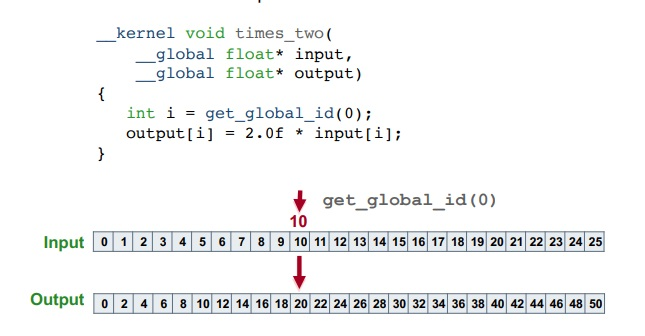
\includegraphics[scale=0.7]{images/kernel.jpg}
\caption{Kernel működése. \cite{opencl_origink}}
\label{fig:kernel}
\end{figure}

Az OpenCL specifikáció 4 nagy egységre bontja az architektúrát, ezek a következők \cite{spec_archi}
\begin{itemize}
\item \textbf{Platform Modell} A modell leírja, hogy milyen legyen a platform amin fut az OpenCL. 
\item \textbf{Végrehajtás modell} Ez a modell két elkülönülő egységet definiál, a kerneleket, amik az OpenCL eszközökön hajtódnak végre, és a házigazda programot, ami a házigazdán hajtódik végre. Ezen kívül a modell leírja azt is, hogy a házigazda hogyan irányítja, utasítja az eszközöket a feladataik végrehajtására.
\item \textbf{Memória modell} Itt definiálnak memória területeket,  memória objektum típusokat, absztrakt memória hierarchiát, megosztott virtuális memóriát.Leírják hogy az OpenCL által használt memória viselkedését, hogy az OpenCL program különböző egységei mely memóriaterületekhez férnek hozzá.
\item \textbf{Programozási modell} Az egyidejűségi modell hogyan vonatkoztatható a fizikai hardverre.

\end{itemize}

\Section{Platform Modell}
A következő sorokban a platform modellt fogjuk bemutatni \cite{spec_platform} :

A platform modell egy házigazdából áll, ami össze van kötve egy vagy több OpenCL eszközhöz. Az OpenCL eszköz több CU-ra (\ref{fig:platform_modell} ábra), számítási egységre van felosztva, amik még tovább vannak osztva PE-kre, processzelő elemekre. A számítási feladatok ezekben az elemekben valósulnak meg. A házigazda parancsokat küld az eszközöknek amik mindent megtesznek hogy végrehajtsák őket, az adatokat a memórián keresztül kapják meg. 

Fejlesztők a belső programokat létrehozhatják C nyelven írt OpenCL forrás stringként, SPIR-V közbülső nyelvi programként, vagy bináris objektumokként, az OpenCL platform biztosít egy fordítót ami lefordítja ezeket futtatható program objektummá. Ez a fordító lehet online, ami a házigazda program futása alatt működik az alapértelmezett API-k használatával, vagy offline, ami a házigazda programon kívül működik platform specifikus módszerekkel.

Az OpenCL 2 féle platform profilt definiál, teljes profilt, és beépített profilt. A teljes profilban lennie kell online fordítónak, a beépített profilban viszont nem kötelező.

\begin{figure}[h]
\centering
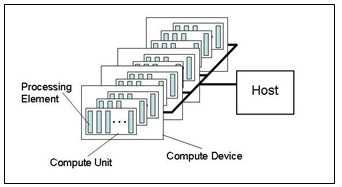
\includegraphics[scale=1.0]{images/platform_modell.jpg}
\caption{Platform modell. \cite{spec_platform}}
\label{fig:platform_modell}
\end{figure}

\Section{Végrehajtás modell}
Ez a rész a végrehajtás modelljét vizsgálja \cite{spec_exec}.

A tényleges párhuzamos munkára a kerneleken kerül sor. A kernel egy a házigazda által precízen menedzselt környezetben, kontextusban fut, aminek részei az eszközök, kernel objektumok, program objektumok, és memória objektumok. Az eszközök 1 vagy több OpenCL platform által megvilágított eszköz, kernel objektumok igazából OpenCL metódusok, amik az OpenCL eszközökön futnak, program objektumok, a program forrás és futtatható állomány amik implementálják a kernelt, a memória objektumok pedig az OpenCL eszközök és a házigazda által látható változók, amiken a kernel példányai dolgoznak.

A házigazda egy eszközzel egy parancs soron keresztül kommunikál, minden eszköznek saját parancs sora van. Egy ilyen parancs 3 kategóriába eshet:
\begin{itemize}
\item\textbf{Kernel sorba állító parancs} Mint a neve is sugallja, besorol egy kernelt egy eszközhöz végrehajtásra.
\item\textbf{Memória parancs} Adatátvitel a házigazda és az eszköz memória között, vagy memória hozzárendelés.
\item\textbf{Szinkronizációs parancs} Explicit szinkronizációs pontok amik meghatároznak egy sorrendiséget.
\end{itemize}
Minden parancs 6 állapoton megy át:
\begin{enumerate}
\item\textbf{Besorolt} A parancs be van sorolva egy parancs sorba.
\item\textbf{Benyújtott} A parancs el van távolítva a parancs sorból, és be van adva eg eszköznek végrehajtás céljából.
\item\textbf{Felkészült} A parancs végrehajtásához szükséges összes előfeltétel teljesült, a parancs ütemezve van végrehajtásra.
\item\textbf{Futó} A parancs végrehajtása elkezdődött.
\item\textbf{Befejezett} A parancs végrehajtása befejeződött.
\item\textbf{Elkészült} A parancs és a gyerek parancsai mind befejeződtek, és a velük kapcsolatos esemény objektum állapota .
\end{enumerate}

\Section{Memória Modell}
A memória modellnek pontosan le kell tudnia definiálni hogy a memóriában lévő értékek hogyan működnek, hogy a fejlesztő helyesen tudja megalkotni a programját. A memória modellnek 4 része van, memória területek, memória objektumok, megosztott virtuális memória, és konzisztencia modell \cite{spec_mem}.

\textbf{A memória terület} az a memória, ami látható a házigazda és az eszközei számára. 2 nagyobb részre van osztva, házigazda memóriára és eszköz memóriára. Az eszköz memória további 4 részre bontható:
\begin{itemize}
\item\textbf{Globális memória} Olyan memória terület amit az összes munka csoport szabadon elér.
\item\textbf{Konstans memória} Ez a terület nem változik a végrehajtás alatt, a házigazda ide helyez memória objektumokat.
\item\textbf{Helyi memória} Munka csoporthoz lokális memória terület
\item\textbf{Privát memória} Munka elemhez tartozó memória terület.
\end{itemize}
\textbf{Memória Objektumok} a globális memória tartalma. 3 fajtájuk van:
\begin{itemize}
\item\textbf{Buffer} Folytonos memória adatok tárolására. Az adatok lehetnek beépített típusok mint integer vagy double, vagy saját típusok is
\item\textbf{Kép} Olyan memória objektum ami képek tárolására szolgál, amik lehetnek akár 3 dimenziósak is.
\item\textbf{Cső}Ez szinte a bashből megismert csővezeték 2 véggel, azzal a tulajdonsággal, hogy a végpontokkal egyszerre csak 1 kernel példány használhat.
\end{itemize}

\Section{OpenCL C nyelvi sajátosságok példák}
Az OpenCL hoz némi újdonságot a nyelvbe, ezek közül mutatok be néhány fontosabbat \cite{opencl_c}
\begin{itemize}
\item\textbf{\_\_ kernel} Egy metódust kernelként azonosít, hasonlóan a main() függvényhez. Egy ilyen kernel hozzáfér más kernel oldali funkciókhoz.
\item\textbf{Memória területek azonosítói} \_\_ global, \_\_ constant, \_\_ local, \_\_ private, a fent említett memóriaterületek azonosítói. Kernel argumentumokhoz szükségesek.
\item\textbf{szinkronizációs funkciók} Sorompók, amiket minden munka elemnek el kell érnie hogy folytathassák a munkájukat, és memória kerítések, amik sorrendezésre adnak lehetőséget.
\end{itemize}

\Section{Egy házigazda program felépítése}
Egy házigazda program egyszerű lépések sorozatából áll \cite{opencl_host}.

\begin{enumerate}
\item Első lépésként definiálni, szerezni kell egy \textbf{platformot}, amin majd fut az OpenCL program. 

\texttt{clGetPlatformIDs(1, \&cpPlatform, NULL)}
\item Ezután meg kell keresni a platformban fellelhető \textbf{OpenCL eszközök}et, és kiválasztani egy vagy több eszközt.

\texttt{clGetDeviceIDs(cpPlatform, CL\_DEVICE\_TYPE\_GPU,1,\&device\_id, NULL)}
\item Harmadikként létre kell hozni egy \textbf{környezet}et, kontextust az OpenCL program számára.

\texttt{clCreateContext(0, 1, \&device\_id, NULL, NULL, \&err)}
\item Negyedik lépés a \textbf{parancs sor} létrehozása.

\texttt{clCreateCommandQueue(context, device\_id, 0, \&err)}
\item Ezután létre kell hozni az \textbf{OpenCL program}ot és felépíteni, lehetőleg egy .cl forrásfájlból.

\texttt{clCreateProgramWithSource(context, 1,(const char **) \&kernelSource\\ , NULL,\&err)}
\newline
\texttt{clBuildProgram(program, 0, NULL, NULL, NULL, NULL)}
\item Létre kell hozni azokat a \textbf{memória objektumok}at, amiket az OpenCL inputként és outputként fog használni.

\texttt{clCreateBuffer(context, CL\_MEM\_READ\_ONLY, bytes, NULL, NULL)}
\item Most már nincs más dolgunk mint létrehozni a \textbf{kernel}t és lefuttatni.

\texttt{clCreateKernel(program, "vecAdd", \&err)}
\item A program futásának befejeztével illendő \textbf{felszabadítani a használt memóriákat}.

\texttt{clReleaseKernel(kernel)}
\end{enumerate}
	
\Section{Eddigi eredmények: M2S-Visual eszköz}
Fontos megemlíteni az Multi2Sim-Visual-t \cite{m2s}. Az M2S egy szimulátor amit abból a célból készítettek, hogy új hardvert lehessen tesztelni prototípus építése nélkül, ez egy heterogén CPU GPU szimulátor, benchmarkokkal kiegészítve. Mivel ekkor egy roppant pontos és kifinomult szimulátorban fut a program, pontosan nyomon lehet követni a program futását. Ehhez készítettek egy Bostoni egyetemen egy vizualizációs keretrendszert az M2S-Visualt \cite{m2sv}. Ez az eszköz képes megmutatni hogy melyik processzor magon milyen kontextus fut, azon belül milyen processzor instrukciók aktívak, vagy hogy a GPU-n hány számítási egység van, azokon belül milyen munka csoportok vannak, vagy akár hogy milyen memória hierarchia áll fenn a gyorsítótárakban.
Hiányossága az eszköznek, hogy csak a pillanatnyi állapotot mutatja, és igazából azt se teljesen vizuálisan hanem inkább táblázatos formákban (\ref{fig:m2svf} ábra).

\begin{figure}[h]
\centering
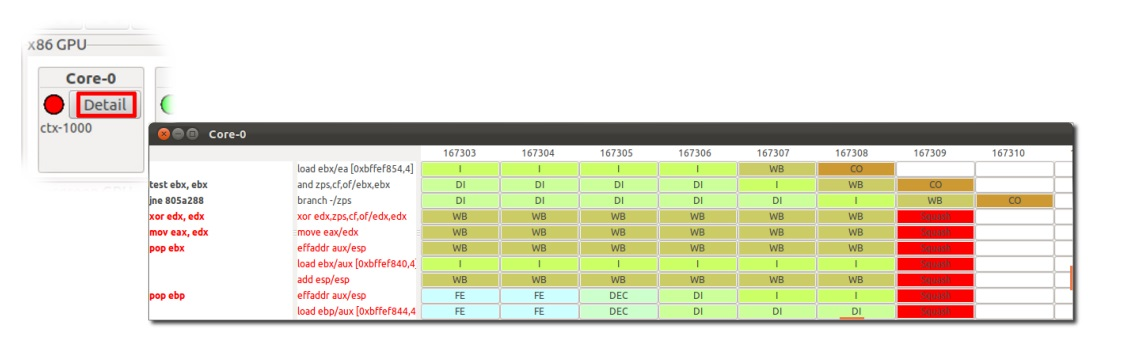
\includegraphics[scale=0.5]{images/m2sv2.jpg}
\caption{M2S-Visual egy idő diagramja. \cite{m2sv}}
\label{fig:m2svf}
\end{figure}

%\Section{Tartalom és felépítés}
%
%A fejezet tartalma témától függően változhat. Az alábbiakat attól függően különböző arányban tartalmazhatják.
%\begin{itemize}
%\item Irodalomkutatás. Amennyiben a dolgozat egy módszer kidolgozására, kifejlesztésére irányul, akkor itt lehet részletesen végignézni (módszertani vagy időrendi bontásban), hogy az eddigiekben milyen eredmények születtek a témakörben.
%\item Technológia. Mivel jellemzően kutatásról vagy szoftverfejlesztésről van szó, ezért annak a jellemző elemeit, technikai részleteit itt kell bemutatni.
%Ez tehát egy módszeres bevezetés ahhoz, hogy ha valaki nem jártas a témakörben, akkor tudja, hogy a dolgozat milyen aktuálisan elérhető eredményeket, eszközöket használt fel.
%\item Piackutatás. Bizonyos témáknál új termék vagy szolgáltatás kifejlesztése a cél.
%Ekkor érdemes annak alaposan utánanézni, hogy aktuálisan milyen eszközök érhetők el a piacon.
%Ez szoftverek esetében a hasonló alkalmazások bemutatását, táblázatos formában történő összehasonlítását jelentheti.
%Szerepelhetnek képek és észrevételek a viszonyításként bemutatott alkalmazásokhoz.
%\item Követelmény specifikáció. Külön szakaszban érdemes részletesen kitérni az elkészítendő alkalmazással kapcsolatos követelményekre.
%Ehhez tartozhatnak forgatókönyvek (\textit{scenario}-k).
%A szemléletesség kedvéért lehet hozzájuk képernyőkép vázlatokat is készíteni, vagy a használati eseteket más módon szemléltetni.
%\end{itemize}

%\Section{Amit csak említés szintjén érdemes szerepeltetni}
%
%Az olvasóról annyit feltételezhetünk, hogy programozásban valamilyen szinten járatos, és a matematikai alapfogalmakkal sem ebben a dolgozatban kell megismertetni.
%A speciális eszközök, programozási nyelvek, matematikai módszerekk és jelölések persze jó, hogy ha említésre kerülnek, de nem kell nagyon belemenni a közismertnek tekinthető dolgokba.
